\documentclass[11pt, a4paper]{article}

\usepackage[T1]{fontenc}
\usepackage[utf8]{inputenc}
\usepackage[polish]{babel}
\usepackage{listings}
\usepackage{mathtools}
\usepackage{blindtext}
\usepackage{scrextend}
\usepackage{graphicx}
\usepackage{amsmath}


\graphicspath{ {./images/} }


\begin{document}

\title{MOwNiT\\Laboratorium 3}
\author{Kacper Janda}
\date{}
\maketitle

\section{Wady klasycznego algorytmu Gaussa}
Rozwiązywanie układu równań liniowych podstawową metodą Gaussa zawodzi gdy na przekątnej macierzy A istnieją zera. Algorytm próbuje wtedy podzielić przez \begin{math} 0 \end{math} co prowadzi do błędu. Algorytm ten nie uwzględnia postaci macierzy A - gdy jest ona macierzą diagonalną algorytm i tak wykonuje wszystkie operacje. Metoda ta posiada złożoność obliczeniową \begin{math} O(n^3) \end{math}. Kolejnym problemem jest fakt powstawania błędów numberycznych spowodowanych dzieleniem przez liczby o małej wartości. Ma to znaczny wpływ na wynik w szczególności w przypadku macierzy źle uwarunkowanych.\\

\section{Optymalizacja algorytmu Gaussa}
Aby zmniejszyć czas potrzebny rozwiązywania układu równań można zastosować rozkład LU macierzy A. Zmniejsza to złożoność obliczeniową o stały współczynnik. Innym sposobem na poprawienie działania algorytmu jest zastosowanie wybierania elementów głównych. Pozwala to zredukować błędy numeryczne.\\

\begin{enumerate}

\item Przykład występowania błędów numerycznych\\

\begin{math}
A = $$
\begin{bmatrix}
10^{-20}&1\\
1&1\\
\end{bmatrix}
$$
\end{math}
\begin{math}
b = $$
\begin{bmatrix}
1\\
2\\
\end{bmatrix}
$$
\end{math}

\begin{center}
    \begin{tabular}{| l | l |}
    \hline
    Metoda & Wynik\\ \hline
    Metoda Gaussa &  \begin{math}
$$
\begin{bmatrix}
0\\
1\\
\end{bmatrix}
$$
\end{math}\\ \hline
    Faktoryzacja LU & \begin{math}
    $$
\begin{bmatrix}
0\\
1\\
\end{bmatrix}
$$
\end{math}\\ \hline
    Skalowana Faktoryzacja LU & \begin{math}
$$
\begin{bmatrix}
1\\
1\\
\end{bmatrix}
$$
\end{math}\\ \hline
    Funkcja biblioteczna& \begin{math}
$$
\begin{bmatrix}
1\\
1\\
\end{bmatrix}
$$
\end{math}\\ \hline
    \end{tabular}
\end{center}
W metodzie używającej skalowanej faktoryzacji LU nie wystąpiły znaczące błędy nueryczne. W przypadku metody Gaussa oraz zwykłej faktoryzacji błędy spowodowały całkowitą zmianę wyniku.

\item Czas wykonywania algorytmów gdy macierz A jest diagonalna.\\
Do pomiarów zostały wykorzystane macierze \begin{math}50\end{math} x \begin{math}50\end{math}

\begin{center}
    \begin{tabular}{| l | l | l |}}
    \hline
    Metoda & Macierz zwykła & Macierz diagonalna\\ \hline
    Metoda Gaussa &  \begin{math}0.008050\end{math}\\ \hline
    Faktoryzacja LU & \begin{math}0.007719\end{math}\\ \hline
    Skalowana Faktoryzacja LU & \begin{math}0.010842\end{math}\\\hline
    Funkcja biblioteczna& \begin{math}0.044250\end{math}\\ \hline
    \end{tabular}
\end{center}

\end{enumerate}

\section{Porównanie wydajności}
\begin{center}
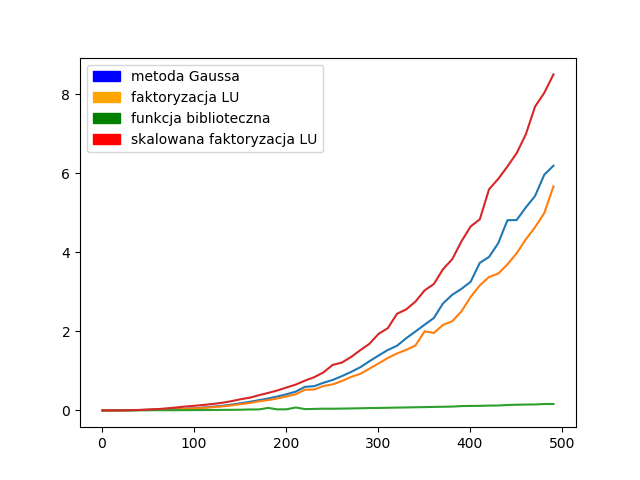
\includegraphics[scale=0.55]{Figure_3}
\end{center}
Wykras pokazuje, że w celu uzyskania jak najlepszej wydajności należy korzystać z funkcji bibliotecznych (w tym przypadku została wykorzystana funkcja 'solve' z biblioteki 'numpy.linalg'). Zgodnie z przewidywaniami wykresy zaimplementowanych funcji przedstawiają złożoność \begin{math} O(n^3) \end{math}

 

\end{document}